\documentclass[aspectratio=169]{beamer}
\usetheme{Frankfurt}
\usecolortheme{seahorse}
\usepackage{graphicx}
\usepackage{amsmath}
\usepackage{booktabs}
\usepackage{pgfgantt}
\usepackage{tikz}
\usepackage{pifont}
\usetikzlibrary{shapes.geometric, arrows, positioning}
\usepackage{xcolor}

\title{Context-Aware Privacy for AR}
\subtitle{Real-Time Selective Anonymization via Egocentric Interaction Detection\\[0.2cm]\textbf{Mid-Review Presentation}}
\setbeamertemplate{headline}{}
\renewcommand{\insertshorttitle}{}
\author[]{Akash Abeywickrame \\ S/20/302 \\ Supervisor: Dr.\ Hakim Usoof}
\institute[UOP]{Department of Statistics and Computer Science \\ Faculty of Science \\ University of Peradeniya}
\date{June 2026}

\setbeamertemplate{author in head/foot}{}
\newcommand{\regno}{S/20/302}
\setbeamertemplate{footline}{
  \leavevmode\hbox{%
    \begin{beamercolorbox}[wd=.33\paperwidth,ht=2.5ex,dp=1ex,leftskip=0.4cm]{author in head/foot}
      \textbf{\regno}
    \end{beamercolorbox}%
    \begin{beamercolorbox}[wd=.34\paperwidth,ht=2.5ex,dp=1ex,center]{author in head/foot}
      \textbf{CSC 4996}
    \end{beamercolorbox}%
    \begin{beamercolorbox}[wd=.33\paperwidth,ht=2.5ex,dp=1ex,rightskip=0.4cm]{date in head/foot}
      \insertframenumber{} / \inserttotalframenumber
    \end{beamercolorbox}%
  }
}
\newcommand{\done}{\textcolor{green!60!black}{\ding{51}}}
\newcommand{\pending}{\textcolor{orange}{\ding{109}}}

\begin{document}

% ---- Title ----
\begin{frame}
  \titlepage
\end{frame}

\begin{frame}{Agenda}
  \tableofcontents
\end{frame}

% ==================================================
\section{Introduction and Problem}

\begin{frame}{Introduction and Problem}
\begin{columns}[T]
\begin{column}{0.50\textwidth}
  \begin{block}{The Problem}
    AR glasses (Meta Ray-Ban, Snap Spectacles) record \textbf{continuous egocentric video} of bystanders without consent.
  \end{block}
  \vspace{0.4cm}
  \textbf{Why current approaches fail:}
  \begin{itemize}\setlength{\itemsep}{0.25cm}
    \item[\textcolor{red}{\ding{55}}] \textbf{Blanket blur} — destroys AR utility
    \item[\textcolor{red}{\ding{55}}] \textbf{LED indicator} — notifies but does not protect
    \item[\textcolor{red}{\ding{55}}] \textbf{Cloud systems} — latency unacceptable on wearables
  \end{itemize}
\end{column}
\begin{column}{0.46\textwidth}
  \begin{alertblock}{Research Question}
    How to \textbf{automatically} distinguish a \textbf{conversation partner} from a \textbf{bystander} and blur only the stranger — \textbf{in real time on a CPU-only edge device}?
  \end{alertblock}
  \vspace{0.5cm}
  \begin{table}
    \small\renewcommand{\arraystretch}{1.3}
    \begin{tabular}{lc}
    \toprule
    \textbf{Metric} & \textbf{Target} \\
    \midrule
    Throughput    & 20--28 FPS \\
    Privacy (PSR) & $\geq$ 95\% \\
    Utility (IPR) & $\geq$ 93\% \\
    \bottomrule
    \end{tabular}
  \end{table}
\end{column}
\end{columns}
\end{frame}

% ==================================================
\section{Literature Review and Research Gap}

\begin{frame}{Literature Review — AR Privacy}
\begin{columns}[T]
\begin{column}{0.48\textwidth}
  \textbf{Privacy Problem}
  \vspace{0.15cm}
  \begin{itemize}\setlength{\itemsep}{0.3cm}
    \item \textbf{O'Hagan et al.\ (2023)} — AR users unaware of bystander implications; no built-in protection in consumer devices
    \item \textbf{Khan et al.\ (2021)} — Wearable cameras need context-aware privacy; generic blurring is the key shortfall
    \item \textbf{Costa et al.\ (2025)} — SafeAR: policy-based AR privacy framework; requires server-side processing
  \end{itemize}
\end{column}
\begin{column}{0.48\textwidth}
  \textbf{Existing Technical Solutions}
  \vspace{0.15cm}
  \begin{itemize}\setlength{\itemsep}{0.3cm}
    \item \textbf{Corbett et al.\ (2023)} — BystandAR: depth + gaze bystander detection; tethered workstation only, not on-device
    \item \textbf{Meta EgoBlur (2023)} — Batch face anonymization for Ego4D dataset; offline processing, not real-time
    \item \textbf{Karakostas et al.\ (2024)} — Edge AR inference on low-power devices; face privacy not addressed
  \end{itemize}
\end{column}
\end{columns}
\end{frame}

\begin{frame}{Literature Review — Interaction Detection Cues}
\begin{columns}[T]
\begin{column}{0.50\textwidth}
  \textbf{Key Interaction Signals from Literature}
  \vspace{0.15cm}
  \begin{itemize}\setlength{\itemsep}{0.3cm}
    \item \textbf{Proximity} — Face area ratio correlates strongly with direct conversation
    \item \textbf{Centrality} — Wearers face their conversation partners; centre-bias in egocentric video
    \item \textbf{Head-pose yaw} — Face oriented toward camera ($|\text{yaw}|<45^\circ$) is the strongest single indicator
    \item \textbf{Visual VAD} — Lip motion variance detects active speech without audio
    \item \textbf{Temporal hysteresis} — Momentary cue changes should not flip labels
  \end{itemize}
\end{column}
\begin{column}{0.46\textwidth}
  \begin{block}{Multi-Cue Fusion}
    Single cues are unreliable in crowded scenes. Literature supports a \textbf{sequential fail-fast pipeline}: cheap cues first, expensive cues only when needed.
  \end{block}
  \vspace{0.4cm}
  \textbf{Key gaps identified:}
  \begin{itemize}\setlength{\itemsep}{0.2cm}
    \item No system combines all four cues on CPU-only hardware
    \item No public dataset with per-face interaction labels for egocentric video
  \end{itemize}
\end{column}
\end{columns}
\end{frame}

\begin{frame}{Research Gap}
\begin{columns}[T]
\begin{column}{0.48\textwidth}
  \begin{block}{What Exists}
    \begin{itemize}\setlength{\itemsep}{0.15cm}
      \item Offline blanket anonymization
      \item Cloud-based identity recognition
      \item Workstation-dependent interaction detection
      \item Theoretical privacy policy frameworks
    \end{itemize}
  \end{block}
  \vspace{0.3cm}
  \begin{alertblock}{What is Missing}
    \begin{itemize}\setlength{\itemsep}{0.15cm}
      \item Real-time edge bystander/partner discrimination
      \item Per-face interaction labels dataset
      \item Privacy–utility trade-off evaluation
    \end{itemize}
  \end{alertblock}
\end{column}
\begin{column}{0.48\textwidth}
  \vspace{0.3cm}
  \begin{block}{How This Work Fills the Gap}
    \renewcommand{\arraystretch}{1.4}
    \begin{tabular}{p{2.5cm}p{2.5cm}}
    \toprule
    \textbf{Gap} & \textbf{Our Contribution} \\
    \midrule
    Real-time edge     & CPU-only pipeline \\
    Interaction cues   & 4-cue sequential classifier \\
    Novel dataset      & 21-video annotated GT \\
    Privacy evaluation & PSR, IPR, F1-score \\
    \bottomrule
    \end{tabular}
  \end{block}
\end{column}
\end{columns}
\end{frame}

% ==================================================
\section{Research Objectives}

\begin{frame}{Research Objectives}
\begin{columns}[T]
\begin{column}{0.52\textwidth}
  \begin{block}{Primary Objective}
    A \textbf{real-time CPU-only} AR privacy system that \textbf{selectively blurs bystanders} while \textbf{preserving interaction partners}.
  \end{block}
  \vspace{0.4cm}
  \begin{enumerate}\setlength{\itemsep}{0.3cm}
    \item[\textbf{O1}] Lightweight face detection and multi-face tracking (YOLOv8n + SORT)
    \item[\textbf{O2}] Multi-cue classifier: proximity, centrality, head-pose yaw, V-VAD
    \item[\textbf{O3}] Novel ground-truth dataset: per-face labels for 21 egocentric videos
    \item[\textbf{O4}] Evaluation: PSR $\geq$ 95\%, IPR $\geq$ 93\%, FPS $\geq$ 20 on Raspberry Pi 5
  \end{enumerate}
\end{column}
\begin{column}{0.44\textwidth}
  \vspace{0.4cm}
  \begin{table}
    \renewcommand{\arraystretch}{1.45}
    \small
    \begin{tabular}{clc}
    \toprule
    & \textbf{Task} & \textbf{Status} \\
    \midrule
    O1 & Detection \& Tracking  & \done \\
    O2 & 2-cue classifier (2a)  & \done \\
    O2 & 4-cue pipeline (2b)    & \pending \\
    O3 & Ground-truth dataset   & \pending \\
    O4 & Evaluation             & \pending \\
    \bottomrule
    \end{tabular}
  \end{table}
\end{column}
\end{columns}
\end{frame}

% ==================================================
\section{Proposed Methodology}

\begin{frame}{Proposed Methodology — System Architecture}
\begin{columns}[c]
\begin{column}{0.38\textwidth}
\begin{center}
\resizebox{!}{0.80\textheight}{%
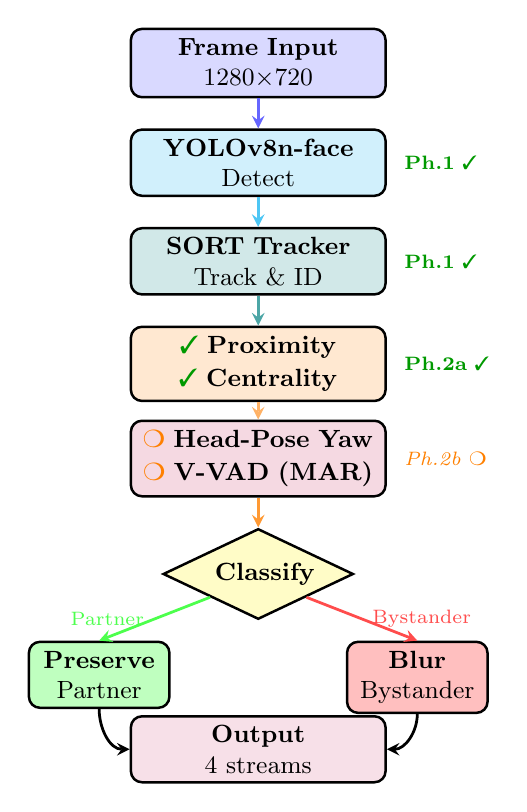
\begin{tikzpicture}[
    node distance=0.38cm,
    box/.style={rectangle, draw, rounded corners, text width=3.0cm, align=center,
                minimum height=0.68cm, font=\small, line width=0.9pt},
    cuebox/.style={rectangle, draw, rounded corners, text width=3.0cm, align=center,
                   minimum height=0.75cm, font=\small, line width=0.9pt},
    dec/.style={diamond, draw, aspect=2.1, text width=1.1cm, align=center,
                font=\small, line width=0.9pt},
    br/.style={rectangle, draw, rounded corners, text width=1.55cm, align=center,
               minimum height=0.65cm, font=\small, line width=0.9pt},
    ph/.style={font=\scriptsize, align=left},
    arr/.style={->, >=stealth, line width=1.0pt}
]

\node[box, fill=blue!15]  (in)  {\textbf{Frame Input}\\1280$\times$720};

\node[box, fill=cyan!18,  below=of in]  (det) {\textbf{YOLOv8n-face}\\Detect};
\node[ph, right=0.1cm of det] {\textcolor{green!60!black}{\textbf{Ph.1} \done}};

\node[box, fill=teal!18,  below=of det] (trk) {\textbf{SORT Tracker}\\Track \& ID};
\node[ph, right=0.1cm of trk] {\textcolor{green!60!black}{\textbf{Ph.1} \done}};

\node[cuebox, fill=orange!18, below=of trk] (ca)
  {\done\ \textbf{Proximity}\\[1pt]\done\ \textbf{Centrality}};
\node[ph, right=0.1cm of ca] {\textcolor{green!60!black}{\textbf{Ph.2a} \done}};

\node[cuebox, fill=purple!15, below=0.22cm of ca] (cb)
  {\pending\ \textbf{Head-Pose Yaw}\\[1pt]\pending\ \textbf{V-VAD (MAR)}};
\node[ph, right=0.1cm of cb] {\textcolor{orange}{\textit{Ph.2b} \pending}};

\node[dec, fill=yellow!22, below=0.38cm of cb] (clf) {\textbf{Classify}};

\node[br, fill=green!25, below left=0.55cm and 0.5cm of clf]  (keep)
  {\textbf{Preserve}\\Partner};
\node[br, fill=red!25,   below right=0.55cm and 0.5cm of clf] (blur)
  {\textbf{Blur}\\Bystander};

\node[box, fill=purple!12, below=1.2cm of clf] (out)
  {\textbf{Output}\\4 streams};

\draw[arr, blue!60]   (in)  -- (det);
\draw[arr, cyan!70]   (det) -- (trk);
\draw[arr, teal!70]   (trk) -- (ca);
\draw[arr, orange!60] (ca)  -- (cb);
\draw[arr, orange!80] (cb)  -- (clf);
\draw[arr, green!70]  (clf.south west)
      -- node[left,font=\scriptsize]{Partner}   (keep.north);
\draw[arr, red!70]    (clf.south east)
      -- node[right,font=\scriptsize]{Bystander}(blur.north);
\draw[arr] (keep.south) to[out=-90,in=180] (out.west);
\draw[arr] (blur.south) to[out=-90,in=0]   (out.east);

\end{tikzpicture}
}
\end{center}
\end{column}
\begin{column}{0.58\textwidth}
  \begin{itemize}\setlength{\itemsep}{0.30cm}
    \item \textbf{Phase 1 \done} — YOLOv8n-face (conf $\geq$0.45, max 20 faces) + SORT tracker. Stable \texttt{track\_id} per face. CPU-only.
    \item \textbf{Phase 2a \done} — Face area ratio $\geq$0.012 AND centre distance $\leq$0.45 $\Rightarrow$ partner. Temporal hysteresis + INTERACT\_LATCH.
    \item \textbf{Phase 2b \pending} — MediaPipe 468-landmark yaw estimation. MAR variance for lip-movement speech detection.
    \item \textbf{Output} — 4 streams: debug, selective, blanket, clean. Bystanders blurred (Gaussian $\sigma$=51).
  \end{itemize}
\end{column}
\end{columns}
\end{frame}

% ==================================================
\section{Data}

\begin{frame}{Dataset}
\begin{columns}[T]
\begin{column}{0.48\textwidth}
  \begin{table}
    \renewcommand{\arraystretch}{1.5}
    \begin{tabular}{lcc}
    \toprule
    \textbf{Category} & \textbf{Videos} & \textbf{Type} \\
    \midrule
    Interaction & 14 & Face-to-face \\
    Bystander   &  7 & Walking past \\
    \midrule
    \textbf{Total} & \textbf{21} & 30 FPS egocentric \\
    \bottomrule
    \end{tabular}
  \end{table}
  \vspace{0.4cm}
  \begin{itemize}\setlength{\itemsep}{0.28cm}
    \item \textbf{Source:} Ego4D + curated clips
    \item \textbf{Resolution:} 1280 $\times$ 720 px, head-mounted
    \item \textbf{Processed:} \texttt{video1.mp4} — 4,879 frames, 94 tracks
  \end{itemize}
\end{column}
\begin{column}{0.48\textwidth}
  \begin{alertblock}{Novel Annotation (Created from Scratch)}
    No public dataset has per-face interaction/bystander labels for egocentric video.
  \end{alertblock}
  \vspace{0.35cm}
  \textbf{Labelling Rule:}\\
  If person \textit{ever} talks to wearer $\Rightarrow$ \textbf{partner (1)}\\
  Never interacts $\Rightarrow$ \textbf{bystander (0)}
  \vspace{0.35cm}
  \begin{itemize}\setlength{\itemsep}{0.2cm}
    \item Blind annotation — numbered faces, no model labels
    \item Cohen's $\kappa$ for inter-annotator agreement
    \item Majority vote $\Rightarrow$ final ground truth
  \end{itemize}
\end{column}
\end{columns}
\end{frame}

% ==================================================
\section{Current Progress}

\begin{frame}{Phase 1 — Detection and Tracking \done}
\begin{columns}[T]
\begin{column}{0.44\textwidth}
  \textbf{YOLOv8n-face}
  \begin{itemize}\setlength{\itemsep}{0.2cm}
    \item Confidence $\geq 0.45$, max 20 faces/frame
    \item Fully local — no GPU, no cloud
  \end{itemize}
  \vspace{0.35cm}
  \textbf{SORT Tracker}
  \begin{itemize}\setlength{\itemsep}{0.2cm}
    \item Kalman Filter + Hungarian algorithm
    \item Stable \texttt{track\_id} per face across frames
  \end{itemize}
  \vspace{0.35cm}
  \begin{block}{Why SORT?}
    \texttt{boxmot}/DeepSORT incompatible with Python 3.13. SORT re-implemented from scratch — sufficient accuracy, cheaper on CPU.
  \end{block}
\end{column}
\begin{column}{0.52\textwidth}
  \begin{figure}
    \includegraphics[width=\textwidth]{output/frame_debug.png}
  \end{figure}
  \centering\small Green = partner preserved \quad Red = bystander blurred
\end{column}
\end{columns}
\end{frame}

\begin{frame}{Phase 2a — Interaction Classifier \done}
\begin{columns}[T]
\begin{column}{0.48\textwidth}
  \begin{block}{Cue 1 — Proximity}
    $\text{area\_ratio} = \dfrac{w_f \cdot h_f}{W \cdot H} \;\geq\; 0.012$\\[4pt]
    Instant override if $\geq$ 4\% (big-face rule)
  \end{block}
  \vspace{0.3cm}
  \begin{block}{Cue 2 — Centrality}
    $d = \dfrac{\sqrt{\Delta x^2 + \Delta y^2}}{\text{half-diag}} \;\leq\; 0.45$
  \end{block}
  \vspace{0.3cm}
  \small \textbf{Hysteresis:} cues hold $\geq 2$ frames before label changes.\\
  \textbf{INTERACT\_LATCH:} once partner — stays partner for full video.
\end{column}
\begin{column}{0.48\textwidth}
  \begin{figure}
    \includegraphics[width=\textwidth]{output/clean_scatter.png}
  \end{figure}
  \centering\small Shaded = both cues pass $\Rightarrow$ partner
\end{column}
\end{columns}
\end{frame}

\begin{frame}{Selective vs.\ Blanket Anonymization}
\begin{columns}[T]
\begin{column}{0.48\textwidth}
  \textbf{Blanket Blur (Baseline)}
  \begin{figure}
    \includegraphics[width=\textwidth]{output/frame_blanket.png}
  \end{figure}
  \centering\small \textcolor{red}{Every face blurred — utility destroyed}
\end{column}
\begin{column}{0.48\textwidth}
  \textbf{Selective Blur — Phase 2a}
  \begin{figure}
    \includegraphics[width=\textwidth]{output/frame_selective.png}
  \end{figure}
  \centering\small \textcolor{green!60!black}{Bystanders blurred, partners preserved}
\end{column}
\end{columns}
\end{frame}

\begin{frame}{Phase 2a — Preliminary Evaluation}
\begin{columns}[T]
\begin{column}{0.48\textwidth}
  \textbf{Accuracy — video1 (66 tracks)}
  \begin{itemize}\setlength{\itemsep}{0.28cm}
    \item PSR (Privacy): \textcolor{orange}{\textbf{87.5\%}} \quad target $\geq$95\%
    \item IPR (Utility): \textcolor{orange}{\textbf{84.6\%}} \quad target $\geq$93\%
    \item F1-Score: \textbf{83.0\%}
    \item Precision: 81.5\% \quad Recall: 84.6\%
    \item 5 privacy leaks (FP) + 4 utility losses (FN)
    \item \textcolor{orange}{$\rightarrow$} Phase 2b expected to close the gap
  \end{itemize}
\end{column}
\begin{column}{0.48\textwidth}
  \textbf{FPS Benchmark — Laptop CPU}
  \begin{itemize}\setlength{\itemsep}{0.28cm}
    \item YOLO detect: \textbf{55.1 ms} (64\% of total)
    \item SORT track: 20.1 ms
    \item Total per frame: \textbf{86.0 ms}
    \item \textbf{11.6 FPS} on laptop CPU \quad target: 20--28 FPS
    \item Bottleneck: YOLO detection
    \item \textcolor{orange}{$\rightarrow$} ONNX quantization + frame-skip planned
  \end{itemize}
\end{column}
\end{columns}
\end{frame}

\begin{frame}{Target Hardware — How Does Our Pipeline Fit?}

\begin{table}
  \centering
  \renewcommand{\arraystretch}{1.55}
  \resizebox{\textwidth}{!}{%
  \begin{tabular}{lccc}
  \toprule
  \textbf{Device} & \textbf{Speed} & \textbf{AI Chip?} & \textbf{Face detect / frame} \\
  \midrule
  Laptop \textit{(baseline)}   & Fast                    & No           & \textbf{55 ms} (measured)      \\
  \textbf{RPi\,5} \textit{(target)} & Moderate            & No           & $\sim$200 ms (estimated)       \\
  Snap Spectacles 5            & Slower CPU than RPi\,5  & \textbf{Yes} & $\sim$70 ms (AI chip helps)    \\
  Meta Ray-Ban 2023            & Very slow               & No           & Not viable ($>$500 ms)         \\
  \bottomrule
  \end{tabular}}
\end{table}

\vspace{0.25cm}
\begin{columns}[T]
\begin{column}{0.54\textwidth}
  \begin{itemize}\setlength{\itemsep}{0.28cm}
    \item \textbf{RPi\,5 CPU is stronger than real glasses} — but glasses have a dedicated AI chip (NPU) that RPi\,5 lacks
    \item RPi\,5 proves the pipeline works \textbf{with no AI chip at all} — the harder case
    \item On real glasses, the AI chip handles the heavy work, so speed is comparable or better
    \item Running \textbf{CPU-only on laptop} simulates this constraint today
  \end{itemize}
\end{column}
\begin{column}{0.42\textwidth}
  \textbf{Reaching 20 FPS on Raspberry Pi 5}
  \vspace{0.1cm}
  \begin{table}
    \renewcommand{\arraystretch}{1.45}\small
    \begin{tabular}{lc}
    \toprule
    \textbf{Step} & \textbf{FPS} \\
    \midrule
    No changes             & $\sim$3  \\
    Compress YOLO model    & $\sim$6  \\
    Skip every 3rd frame   & $\sim$18 \\
    Lower input image size & $\geq$\textbf{20} \\
    \bottomrule
    \end{tabular}
  \end{table}
\end{column}
\end{columns}
\end{frame}

\begin{frame}{Evaluation Infrastructure \done}
\begin{columns}[T]
\begin{column}{0.48\textwidth}
  \textbf{All tools built and tested:}
  \vspace{0.2cm}
  \begin{itemize}\setlength{\itemsep}{0.28cm}
    \item[\done] \texttt{extract\_track\_samples.py} — best crop per track
    \item[\done] \texttt{generate\_annotation\_package.py} — blind numbered frames for human annotators
    \item[\done] \texttt{aggregate\_annotations.py} — Cohen's $\kappa$ + majority-vote GT
    \item[\done] \texttt{evaluate.py} — PSR, IPR, F1, per-stage FPS
  \end{itemize}
\end{column}
\begin{column}{0.48\textwidth}
  \textbf{Accuracy pipeline:}
  \vspace{0.15cm}
  \begin{center}
  \resizebox{0.85\textwidth}{!}{%
  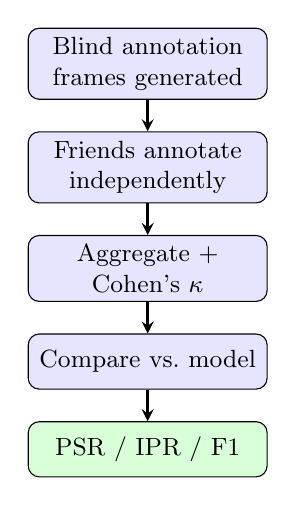
\begin{tikzpicture}[
    node distance=0.4cm,
    pstep/.style={rectangle, draw, fill=blue!10, rounded corners,
                  text width=2.8cm, align=center, font=\small, minimum height=0.7cm},
    arr/.style={->, >=stealth, line width=0.9pt}
  ]
  \node[pstep] (s1) {Blind annotation\\frames generated};
  \node[pstep, below=of s1] (s2) {Friends annotate\\independently};
  \node[pstep, below=of s2] (s3) {Aggregate +\\Cohen's $\kappa$};
  \node[pstep, below=of s3] (s4) {Compare vs.\ model};
  \node[pstep, fill=green!15, below=of s4] (s5) {PSR / IPR / F1};
  \draw[arr] (s1)--(s2); \draw[arr] (s2)--(s3);
  \draw[arr] (s3)--(s4); \draw[arr] (s4)--(s5);
  \end{tikzpicture}
  }
  \end{center}
\end{column}
\end{columns}
\end{frame}

% ==================================================
\section{Remaining Work and Future Directions}

\begin{frame}{Phase 2b — Head-Pose and V-VAD \pending}
\begin{columns}[T]
\begin{column}{0.48\textwidth}
  \begin{block}{Cue 3 — Head-Pose Yaw}
    Estimate rotation from 468 MediaPipe landmarks.\\
    $|\text{yaw}| > 45^\circ$ $\Rightarrow$ bystander (reject before V-VAD)
  \end{block}
  \vspace{0.3cm}
  \begin{block}{Cue 4 — Visual VAD}
    Mouth Aspect Ratio (MAR) variance over time.\\
    High variance = active speech = partner
  \end{block}
  \vspace{0.3cm}
  \small Each cue is a \textbf{fail-fast gate} — fail early = bystander immediately. CPU cost stays low.
\end{column}
\begin{column}{0.48\textwidth}
  \textbf{Complete 4-cue pipeline:}
  \vspace{0.1cm}
  \begin{center}
  \resizebox{0.80\textwidth}{!}{%
  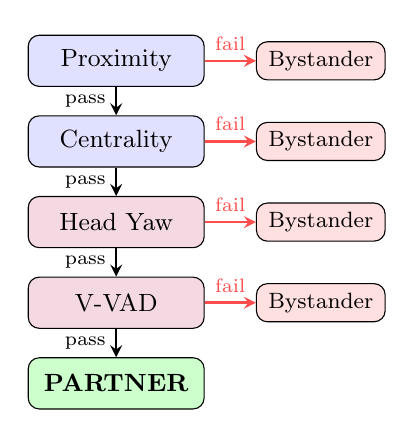
\begin{tikzpicture}[
    node distance=0.36cm,
    s1/.style={rectangle, draw, fill=blue!12, rounded corners,
               text width=2.0cm, align=center, font=\small, minimum height=0.65cm},
    s2/.style={rectangle, draw, fill=purple!15, rounded corners,
               text width=2.0cm, align=center, font=\small, minimum height=0.65cm},
    rej/.style={rectangle, draw, fill=red!12, rounded corners,
                text width=1.4cm, align=center, font=\footnotesize},
    arr/.style={->, >=stealth, line width=0.9pt}
  ]
  \node[s1] (p1) {Proximity};
  \node[s1, below=of p1] (p2) {Centrality};
  \node[s2, below=of p2] (p3) {Head Yaw};
  \node[s2, below=of p3] (p4) {V-VAD};
  \node[s1, fill=green!20, below=of p4] (ok) {\textbf{PARTNER}};

  \node[rej, right=0.65cm of p1] (r1) {Bystander};
  \node[rej, right=0.65cm of p2] (r2) {Bystander};
  \node[rej, right=0.65cm of p3] (r3) {Bystander};
  \node[rej, right=0.65cm of p4] (r4) {Bystander};

  \draw[arr] (p1)--node[left,font=\scriptsize]{pass}(p2);
  \draw[arr] (p2)--node[left,font=\scriptsize]{pass}(p3);
  \draw[arr] (p3)--node[left,font=\scriptsize]{pass}(p4);
  \draw[arr] (p4)--node[left,font=\scriptsize]{pass}(ok);
  \draw[arr,red!70](p1.east)--node[above,font=\scriptsize]{fail}(r1.west);
  \draw[arr,red!70](p2.east)--node[above,font=\scriptsize]{fail}(r2.west);
  \draw[arr,red!70](p3.east)--node[above,font=\scriptsize]{fail}(r3.west);
  \draw[arr,red!70](p4.east)--node[above,font=\scriptsize]{fail}(r4.west);
  \end{tikzpicture}
  }
  \end{center}
  \small \textcolor{blue!70}{Blue = Phase 2a done} \quad \textcolor{purple!70}{Purple = Phase 2b}
\end{column}
\end{columns}
\end{frame}

\begin{frame}{Future Directions — Evaluation Plan}
\begin{columns}[T]
\begin{column}{0.50\textwidth}
  \begin{itemize}\setlength{\itemsep}{0.4cm}
    \item[\pending] Annotate all \textbf{40 videos} and compute Cohen's $\kappa$
    \item[\pending] Implement \textbf{Phase 2b} — head-pose yaw + V-VAD
    \item[\pending] Re-evaluate: Phase 2a vs.\ 2b accuracy and speed
    \item[\pending] \textbf{Raspberry Pi 5} benchmark — FPS on real edge hardware
    \item[\pending] Optimise: ONNX quantization + frame-skipping
  \end{itemize}
\end{column}
\begin{column}{0.46\textwidth}
  \begin{table}
    \renewcommand{\arraystretch}{1.6}\small
    \begin{tabular}{lcc}
    \toprule
    \textbf{Metric} & \textbf{Now} & \textbf{Target} \\
    \midrule
    PSR  & 87.5\%  & $\geq$ 95\% \\
    IPR  & 84.6\%  & $\geq$ 93\% \\
    F1   & 83.0\%  & --- \\
    FPS  & 11.6    & $\geq$ 20 \\
    \bottomrule
    \end{tabular}
  \end{table}
  \vspace{0.2cm}
  \centering\small Phase 2b targets to close all gaps
\end{column}
\end{columns}
\end{frame}

% ==================================================
\section{Timeline}

\definecolor{donecolor}{RGB}{180,180,180}
\definecolor{implcolor}{RGB}{155, 89,182}
\definecolor{datacolor}{RGB}{ 46,204,113}
\definecolor{writecolor}{RGB}{231, 76, 60}

\begin{frame}{Revised Project Timeline}
\begin{center}
\resizebox{\textwidth}{!}{
\begin{ganttchart}[
    hgrid, vgrid,
    x unit=0.9cm, y unit title=0.6cm, y unit chart=0.58cm,
    bar height=0.6, title height=1,
    bar label font=\footnotesize, title label font=\footnotesize,
    bar/.style={fill=gray!30},
  ]{1}{10}
  \gantttitle{Year 2026}{10} \\
  \gantttitle{Jan}{1}\gantttitle{Feb}{1}\gantttitle{Mar}{1}\gantttitle{Apr}{1}
  \gantttitle{May}{1}\gantttitle{\textbf{Jun}}{1}\gantttitle{Jul}{1}
  \gantttitle{Aug}{1}\gantttitle{Sep}{1}\gantttitle{Oct}{1} \\
  \ganttbar[bar/.style={fill=donecolor}]{Proposal \& Literature Review \textnormal{[Done]}}{1}{3} \\
  \ganttbar[bar/.style={fill=donecolor}]{Data Collection \textnormal{[Done]}}{2}{3} \\
  \ganttbar[bar/.style={fill=donecolor}]{Phase 1 — Detection \& Tracking \textnormal{[Done]}}{3}{4} \\
  \ganttbar[bar/.style={fill=donecolor}]{Phase 2a — Decision Layer \textnormal{[Done]}}{4}{5} \\
  \ganttbar[bar/.style={fill=implcolor}]{Phase 2b — Yaw + V-VAD}{6}{7} \\
  \ganttbar[bar/.style={fill=datacolor}]{Ground Truth Annotation}{6}{7} \\
  \ganttbar[bar/.style={fill=implcolor}]{Evaluation \& Pi 5 Benchmarking}{7}{8} \\
  \ganttbar[bar/.style={fill=writecolor}]{Final Report}{8}{10}
\end{ganttchart}
}
\end{center}
\vspace{0.2cm}
{\small
  \textcolor{donecolor}{$\blacksquare$}~Completed \quad
  \textcolor{implcolor}{$\blacksquare$}~Development \quad
  \textcolor{datacolor}{$\blacksquare$}~Annotation \quad
  \textcolor{writecolor}{$\blacksquare$}~Writing \quad
  \textbf{$|$}~Today (June 2026)
}
\end{frame}

% ==================================================
\section{References}
\begin{frame}[allowframebreaks]{References}
\footnotesize
\begin{thebibliography}{99}
  \bibitem{corbett2023}    Corbett et al.\ (2023). \textit{BystandAR: Protecting Bystander Visual Data in AR.} MobiSys.
  \bibitem{ohagan2023}     O'Hagan et al.\ (2023). \textit{Privacy-enhancing technology and everyday AR.} IMWUT.
  \bibitem{khan2021}       Khan et al.\ (2021). \textit{Wearable privacy-preserving egocentric context detection.} UMAP.
  \bibitem{meta2023}       Meta Reality Labs. (2023). \textit{EgoBlur: Privacy-Preserving Egocentric Vision.} arXiv:2308.13093.
  \bibitem{karakostas2024} Karakostas et al.\ (2024). \textit{Real-time wearable AR on the edge.} Virtual Reality.
  \bibitem{costa2025}      Costa et al.\ (2025). \textit{SafeAR: Privacy in AR Applications.} ESOCC.
\end{thebibliography}
\end{frame}

% ---- Thank You ----
\begin{frame}
\centering
\vspace{1.0cm}
{\Huge \textbf{Thank You}}
\vspace{0.8cm}

\normalsize
\textbf{Akash Abeywickrame} \\ S/20/302 \\[0.2cm]
\textit{s20302@sci.pdn.ac.lk}
\vspace{0.8cm}

{\Large \textbf{Q\,\&\,A}}
\end{frame}

\end{document}}

\end{document}
}

\end{document}
